\documentclass[border=3mm,tikz]{standalone}
\usepackage{pgfplots}

\pgfplotsset{compat=1.10}
\usepgfplotslibrary{fillbetween}
\usetikzlibrary{patterns}

\begin{document}

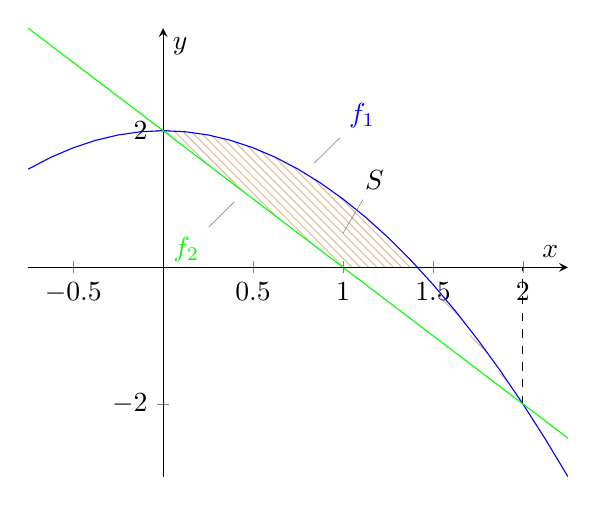
\begin{tikzpicture}
\begin{axis}[axis lines=middle,
            xlabel=$x$,
            ylabel=$y$,
            %enlargelimits,
            %ytick=\empty,
            % xtick={0,1},
            % xticklabels={$x_1$,$x$}
            ]
\addplot[name path=F,blue,domain={-0.75:2.25}] {2-x^2} node[pos=0.3,pin=45:{$f_1$}]{};
\addplot+[mark=none,black,dashed] coordinates {(2,-2)(2,0)};% node[pos=1, above]{$x=2$};
%\addplot+[mark=none,dashed] coordinates {(0,-3)(0,5)} node[pos=1, right]{$x=0$};
\addplot[name path=G,green,domain={-0.75:2.25}] {2-2*x} node[pos=0.4,pin=225:{$f_2$}]{};
\addplot+[name path=H,mark=none,black] coordinates {(0,0)(sqrt(2),0)};

\addplot[pattern=north west lines, pattern color=brown!50]fill between[of=F and G, soft clip={domain=0:1}];
\addplot[pattern=north west lines, pattern color=brown!50]fill between[of=F and H, soft clip={domain=1:2}];
\node[coordinate,pin=70:{$S$}] at (axis cs:1.0,0.5){};
\node[coordinate,pin=30:{$x=0$}] at (axis cs:0,5){};
\end{axis}
\end{tikzpicture}


\end{document}
